

\subsection{Spiral Image Transformer}

    The Spiral Image Transformer, as implied by its name, is a transformer-based model specifically designed to process image data by unrolling pixels in a spiral pattern. This approach stands in contrast to the CIT Model, which processes data using a column-by-column method.

    \begin{figure}[H]
        \centering
        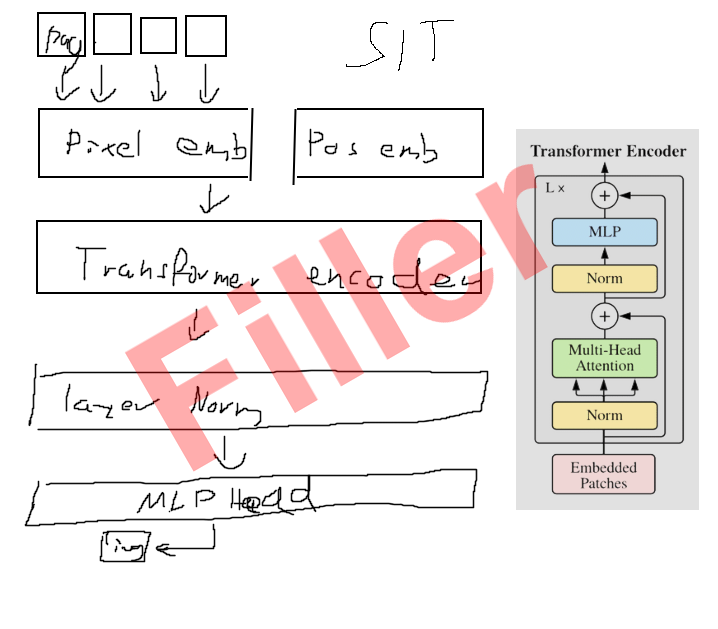
\includegraphics[width=0.8\textwidth]{imgs/SITModel.png}
        \caption{Spiral Image Transformer model structure}
        \label{fig:SpiralImageTransformer}
    \end{figure}

    The visual representation above illustrates the operational steps of the SIT model. Similar to the CIT model, it begins by loading and converting the data. However, it diverges in its method by transforming the data into a spiral format, instead of using the columnar approach. Like its counterpart, this model embeds pixels, from 3 colors to a higher-dimensional embedding space represented by \(N_{\text{EMBD}}\). Positional embeddings are then added. Similar to the CIT model, transformer layers are used to further process the data. The embedded data is finally processed by a (MLP), which converts it back into the original 3-color format. After this step, the spiral-formatted data is restructured into the original image layout.

    \subsubsection{Spiral Data Processing}

    To transform the data, which is loaded by the DataLoader and iterated over, into a spiral format, the width and height dimensions are first squeezed into a single dimension. This resulting tensor has the shape (Batch, Color Channels, Spiral Length). The next step involves indexing the data into the spiral form. For more detailed information on this indexing process, refer to \autoref{fig:spiral_indexing_1}. The restructured tensor is then processed like how the data is handled in the Column Image Transformer model. The following code block illustrates the process used to convert the data into a spiral format.

    \begin{figure}[H]
        \centering
        \begin{lstlisting}[language=Python]
def get_batch(data):
    # Batch_size, Color Channels, Height, Width
    B, C, H, W = data.shape

    spiral_data = torch.zeros_like(data.view(B, C, -1))

    spiral_data[:,:,spiral_indices.flatten()] = data.view(B, C, -1)

    source = spiral_data[:, :, :BLOCK_SIZE]
    label = spiral_data[:, :, 1:BLOCK_SIZE+1]

    source = rearrange(source, 'b c h -> b h c')
    label = rearrange(label, 'b c h -> b h c')

    return source, label
        \end{lstlisting}
        \caption{Python function to get data in a spiral form}
        \label{fig:spiral_indexing_code}
    \end{figure}

    \subsubsection{Spiral generation}
    \label{sec:spiral_generation}
    The conversion of data into a spiral form needs to be highly efficient because the code block will execute for every training step. Therefore, a simple nested for loop is insufficient to rearrange the data into the desired form. In this example, fancy indexing is used to convert the data into a spiral form. Thus, the data tensor is indexed with a flattened two-dimensional tensor containing the indices of the spiral form.

    At the start of the model training script, one indexing spiral is created to be used for all images in the dataset. The following code block illustrates the creation of the spiral index tensor.

\begin{figure}[H]
\centering
\begin{lstlisting}[language=Python]
def create_spiral(n): # n = width and height
    
    matrix = [[0] * n for _ in range(n)] # Initialize n x n matrix

    x, y = 0, 0
    # Direction vectors (right, down, left, up)
    dx = [0, 1, 0, -1]
    dy = [1, 0, -1, 0]
    direction = 0

    for i in range(n * n - 1, -1, -1):  # Start (35 for 6x6)
        matrix[x][y] = i
        nx = x + dx[direction]
        ny = y + dy[direction]

        # Change direction if the next position: out of bounds or filled
        if nx<0 or nx>=n or ny<0 or ny>=n or matrix[nx][ny]!=0:
            direction = (direction + 1) % 4  # Change direction
            nx = x + dx[direction]
            ny = y + dy[direction]

        x, y = nx, ny
    
    return torch.tensor(matrix)
\end{lstlisting}
\caption{Python function to create a spiral index tensor}
\label{fig:spiral_matrix}
\end{figure}

    The code above generates a square matrix of size n by n, then fills it with numbers in a spiral pattern, starting from the outer edge and spiraling inwards clockwise. Each cell of the matrix is assigned a unique number, beginning from the highest value in the top-left corner and decreasing by one with each step along the spiral path until reaching zero at the center or the end of the spiral. The spiral formation is achieved by moving right, then down, then left, then up, and repeating this sequence, adjusting direction whenever the next step would go out of bounds or into a cell that is already been filled.

    The generated spiral index tensor is then used to index the data tensor, effectively converting it into a spiral form. The following image illustrates the process of converting a 7x7 image.
    
    
    \begin{figure}[H]
    \centering
    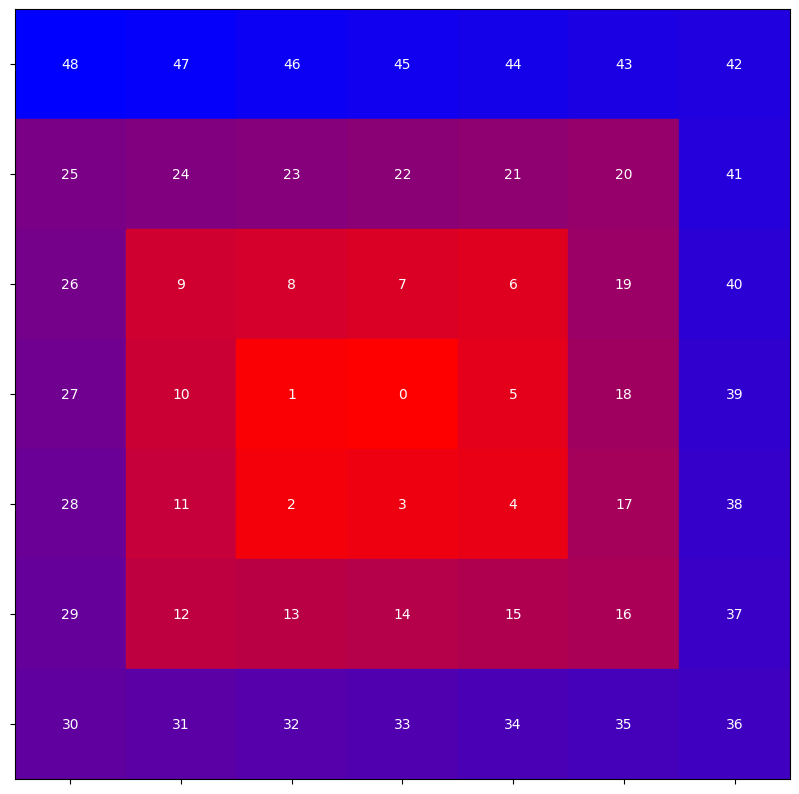
\includegraphics[width=0.6\textwidth]{../code/dataAnalysis/plots/exampleImgs/spiralShowcase1.png}
    \caption{7x7 image with a spiral index overlay}
    \label{fig:spiral_indexing_1}        
    \end{figure}

    \begin{figure}[H]
    \centering
    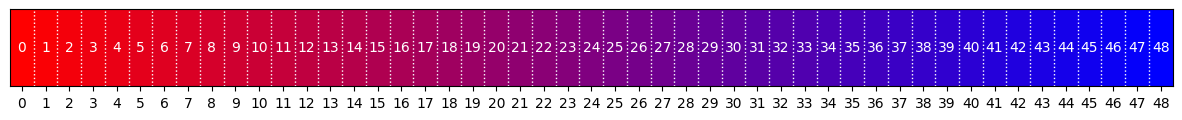
\includegraphics[width=1\textwidth]{../code/dataAnalysis/plots/exampleImgs/spiralShowcase0.png}
    \caption{7x7 Image flattened into the spiral form} 
    \label{fig:spiral_indexing_0}        
    \end{figure}

    As shown in \autoref{fig:spiral_indexing_1}, the pixels of the image are labeled with their respective indices 0, \dots, 48. The image is then unrolled into a single dimension, as shown in \autoref{fig:spiral_indexing_0}. The centering pixel is the first element of the spiral, and the spiral continues counterclockwise from there. In the model script, the dimensions for width and height typically exceed a width of 7, yet the underlying process remains unchanged.



\subsubsection{Model Architecture}

Similar to the CIT model, the addition of positional embeddings is handled in the same manner. This is because the data is transformed into a spiral pattern, allowing the addition of positional embeddings to remain unchanged. Additionally, the transformer layer operates identically. For more information on the transformer layer, see the CIT model \autoref{sec:transformer_CIT}.


\subsubsection{Training the Model}

This model is trained using the Adam optimizer with a learning rate of \(3 \times 10^{-5}\). The loss function used is the Mean Squared Error (MSE) loss. Both training sizes of the model are trained for 4 epochs with a batch size of 8 for the small model and 4 for the big model. The model is trained on the x512 dataset. All the relevant trained SIT models [model 5-6] with their corresponding parameters can be found in detail in the appendix, see \autoref{sec:trained_models_hyperparameters}.

\begin{figure}[H]
    \centering
    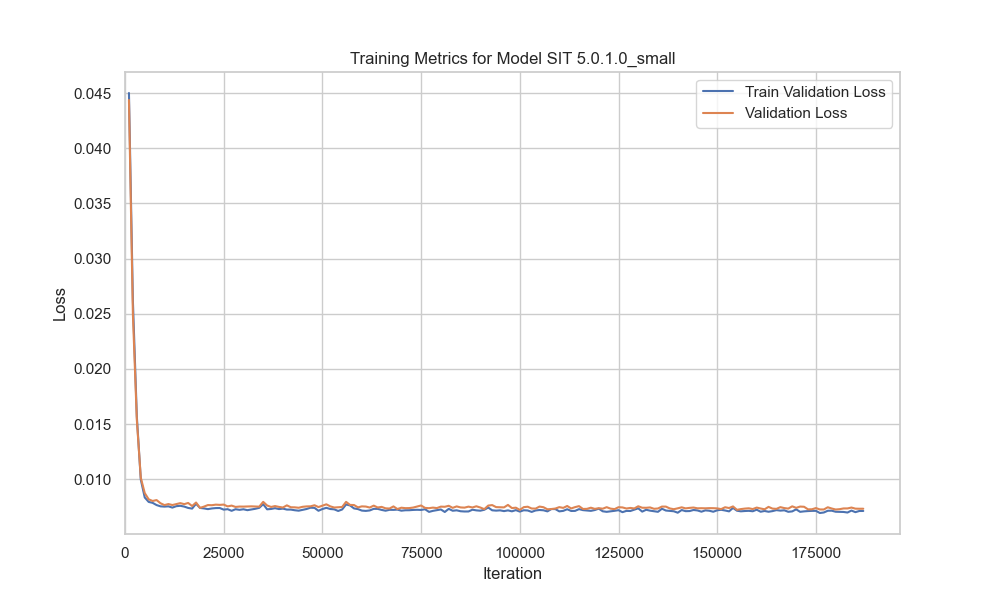
\includegraphics[width=0.9\textwidth]{imgs/Training_Metrics_SIT 5.0.1.0_small.png}
    \caption{Loss plot of the SIT [model 5]}
    \label{fig:Training_Metrics_SITSmall}
\end{figure}

\subsubsection{Experimental Results}

A series of experiments were carried out to assess the capabilities of the Spiral Image Transformer (SIT) model like the CIT Model. The outcomes of these experiments provide insights into the efficacy of the SIT model and highlight potential areas for improvement.

In each of the tests, the end of the seed pixels is marked with a purple pixel indicating the beginning of the generation.

    \begin{itemize}
        \item \textbf{Color test:} To evaluate the color capabilities of the model, a test image with a solid color with a size of 36x36 pixels is provided to the model. The model is then tasked with generating a new image that is 42x42 pixels in width. The test is conducted using two different models, one small and one large.

        \begin{figure}[H]
            \centering
            % First row
            \begin{minipage}{0.40\textwidth}
                \centering
                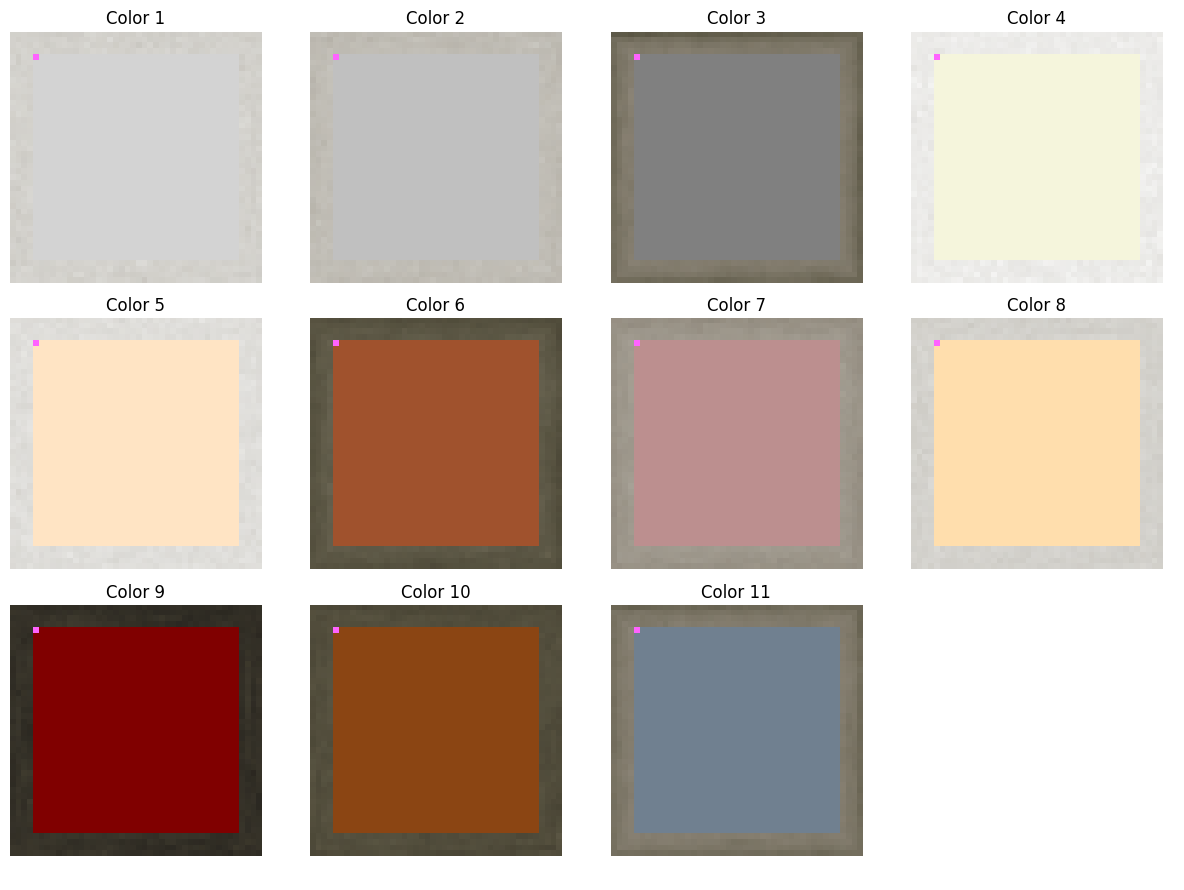
\includegraphics[width=\textwidth]{imgs/ColorTest_5.0.1.0_small.png} 
                \subcaption{[model 5] 5.0.1.0 small}
                \label{fig:test0_1_M4_SIT}
            \end{minipage}
            \hspace{0.05\textwidth}
            \begin{minipage}{0.40\textwidth}
                \centering
                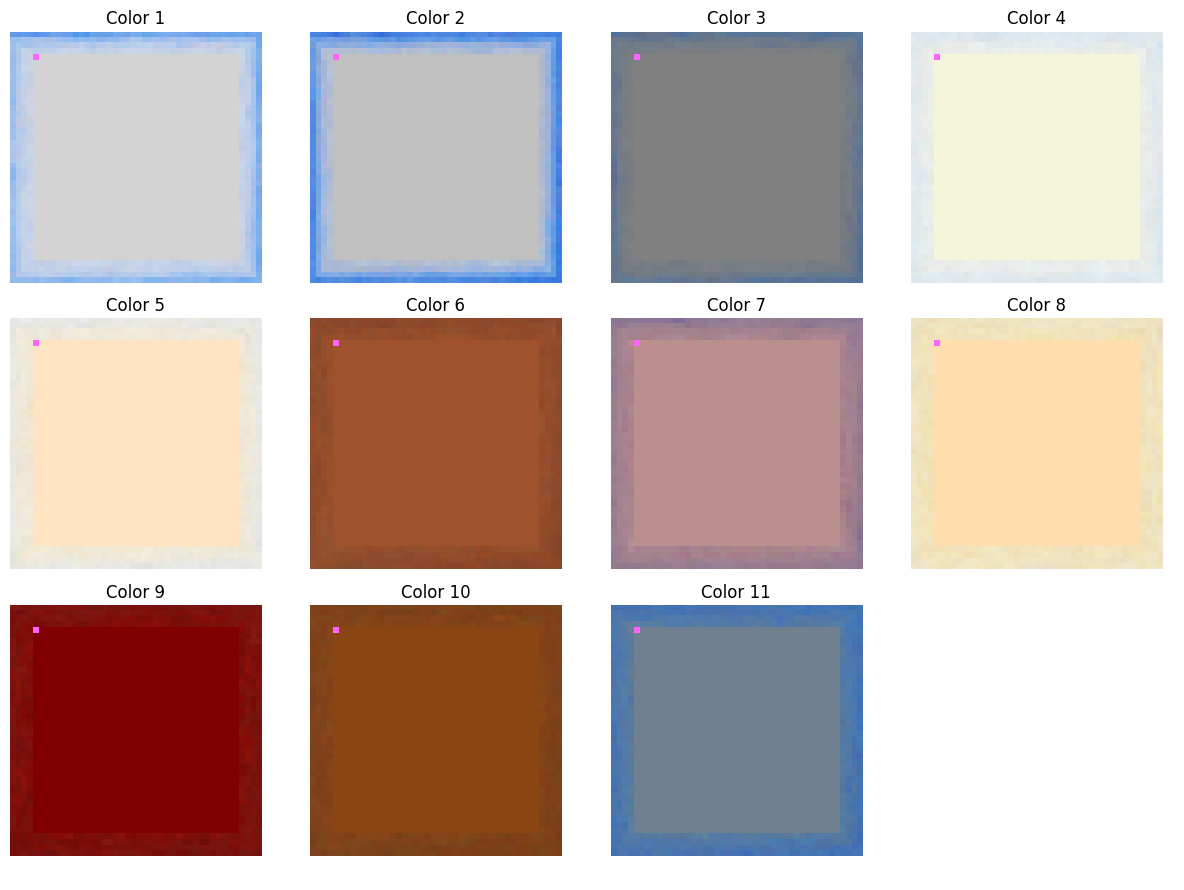
\includegraphics[width=\textwidth]{imgs/ColorTest_5.0.1.0_big.png} 
                \subcaption{[model 6] 5.0.1.0 big}
                \label{fig:test0_2_M5_SIT}
            \end{minipage}
            \caption{Color test with two different model sizes}
        \end{figure}
        
        As depicted in the images above, the smaller model cannot even come close to the desired color output. The larger model performs somewhat better but still struggles to produce the correct color output, especially with the lighter gray shades.
        
        \item \textbf{Image Continuation Test:} The image continuation test is designed to evaluate the model's ability to expand an image. The model is provided with a test image measuring 25 pixels, see \autoref{fig:test2_init_SIT} and is tasked with generating around it to a width of 44 pixels.

        \begin{figure}[H]
            \centering
            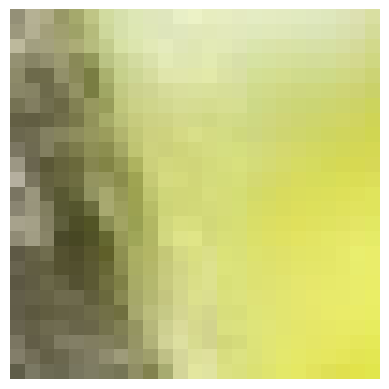
\includegraphics[width=0.3\textwidth]{imgs/ImageTest_5.0.1.0_init.png}
            \caption{Initial test image}
            \label{fig:test2_init_SIT}
        \end{figure}
        
        \begin{figure}[H]
            \centering
            
\includegraphics[width=\textwidth]{imgs/ImageTest_5.0.1.0_flattend.png}
            \caption{Test image flattened into spiral form}
            \label{fig:test2_flattend_SIT}
        \end{figure}
        
        \autoref{fig:test2_flattend_SIT} shows the test image flattened into the spiral form.
        
        \begin{figure}[H]
            \centering
            % First row
            \begin{minipage}{0.48\textwidth}
                \centering
                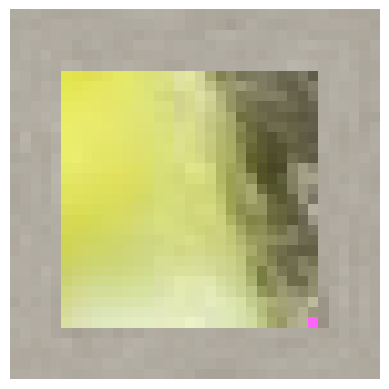
\includegraphics[width=0.8\textwidth]{imgs/ImageTest_5.0.1.0_small.png} 
                \subcaption{[model 5] 5.0.1.0 small}
                \label{fig:test2_1_M4_SIT}
            \end{minipage}
            \hfill
            \begin{minipage}{0.48\textwidth}
                \centering
                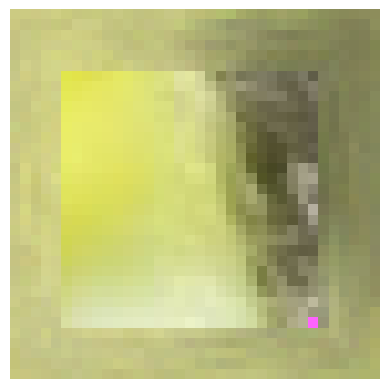
\includegraphics[width=0.8\textwidth]{imgs/ImageTest_5.0.1.0_big.png} 
                \subcaption{[model 6] 5.0.1.0 big}
                \label{fig:test2_2_M5_SIT}
            \end{minipage}
            \caption{Image continuation test with two different model sizes}
            \label{fig:test2_result_SIT}
        \end{figure}
        
        As depicted in \autoref{fig:test2_result_SIT}, the smaller model has difficulty producing the correct color output, focusing primarily on the last gray pixels. In contrast, the larger model performs better, generating a color closer to the desired output. It is important to note that the big model correctly captures that the image should be a light green color on the left side and a gray/dark green color on the right side. This indicates that the model can understand the positional context within the image. However, the model still struggles to generate a clear output.
        

        \item \textbf{Spiral Pattern Test:} The third test evaluates whether the model can accurately generate colors in a rainbow spiral pattern. This test is conducted in a manner very similar to the previous test but provides a more detailed perspective on certain problems. The model starts generating in the upper left corner and continues downwards, then to the right in a counterclockwise motion. The purple pixel indicates the beginning of the generation. The test image is rotated 90 degrees four times to give the model four different starting locations.

        \begin{figure}[H]
            \centering
            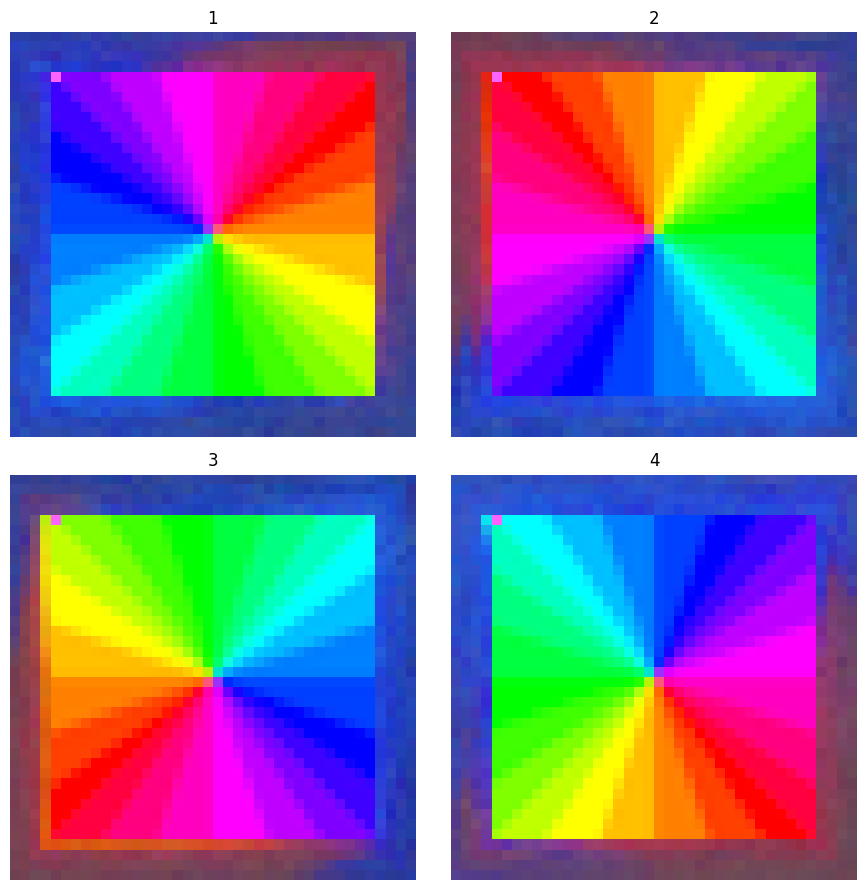
\includegraphics[width=0.7\textwidth]{imgs/RainbowImageTest_5.0.1.0_big.png}
            \caption{Rainbow spiral pattern test SIT [model 6]}
            \label{fig:test3_SIT}
        \end{figure}
        
        As demonstrated in \autoref{fig:test3_SIT}, the model tends to favor the generation of blue or red colors while avoiding yellow, purple, and especially green colors. However, it is noticeable in Image No. 4 that the model generates red accents, although this color is on the opposite side of the starting point. The issues could be due to a lack of training data or the model's size, which needs further investigation.
        

    \end{itemize}

    \subsubsection{Challenges and Limitations}

    As revealed in the experimental section, the Spiral Image Transformer (SIT) model faces difficulties in accurately generating the intended color outputs. This challenge could be anticipated, given that the SIT model's task is inherently more complex than that of the Column Image Transformer (CIT) model. A pattern that progresses one dimensional in a single column is far simpler to learn than one that spirals in two dimensions. The smaller SIT model has an equivalent number of parameters to the smallest CIT model and was trained on an identical dataset, yet its performance is noticeably inferior. Similarly, the larger SIT model holds a parameter count on par with the mid-sized CIT model but falls short in the color tests.

    The limitations experienced by the SIT model could be partially attributed to the insufficiently diverse training dataset. Expanding the dataset, introducing more variance in the training examples, and scaling up the model's complexity could potentially fix its current deficiencies. Moreover, equipping the model with additional contextual data, such as the precise location of a random crop, might improve its capacity for understanding and interpreting the broader context of an image.

    Incorporating a text prompt feature presents could result in a big improvement. By translating descriptive language into visual cues, a text prompt could guide the SIT model toward generating more accurate outputs, potentially reducing or even eliminating the need for seed pixels in some cases.

    Nevertheless, the current iteration of the SIT model is considerably resource-intensive. Its inability to generate multiple pixels parallel translates into lengthy runtimes when operated on consumer-grade GPUs.

